\section{Σύγκριση RNN μοντέλων}

Αρχικά εκπαιδέυτηκαν παράλληλα οι δύο πρώτες περιπτώσεις των RNN που αναφέρθηκαν στο προηγούμενο κεφάλαιο. Από το 1ο διάγραμμα
\ref{f:g1} παρατηρείται ότι κατα την εκπαίδευση έχουμε overfitting απο την 20η εποχή και μετά, ενώ στο δεύτερο διάγραμμα \ref{f:g2} τα RNN 
δυσκολεύονται να ανεβάσουν το accuracy και αυτό φαίνεται απο τα spikes και στα δύο γραφήματα. Στην τρίτη περίπτωση λόγω του overfitting στην 1η προστέθηκε ο l2 για να σταθεροποιηθεί το accuracy, αλλα παρατηρήθηκε όχι μόνο το αντίθετο αλλά το test accuracy/loss έγινε ασταθές όπως φαίνεται και στο διάγραμμα \ref{f:g3}. Στην τελευταία που προσθέσαμε το Batch Normalization παρατηρήθηκαν τα ίδια αποτελέσματα με την 1η περίπτωση.
Γενικά τα Simple RNN είχαν πολύ κακη επίδοση και ήταν πολυ ασταθή σε όλες τις περιπτώσεις. Ακόμα και σε όλο το dataset που εκπαιδεύτηκε παρατηρούνταν τα ίδια αποτελέσματα.


\begin{figure}[ht]
	\centering
	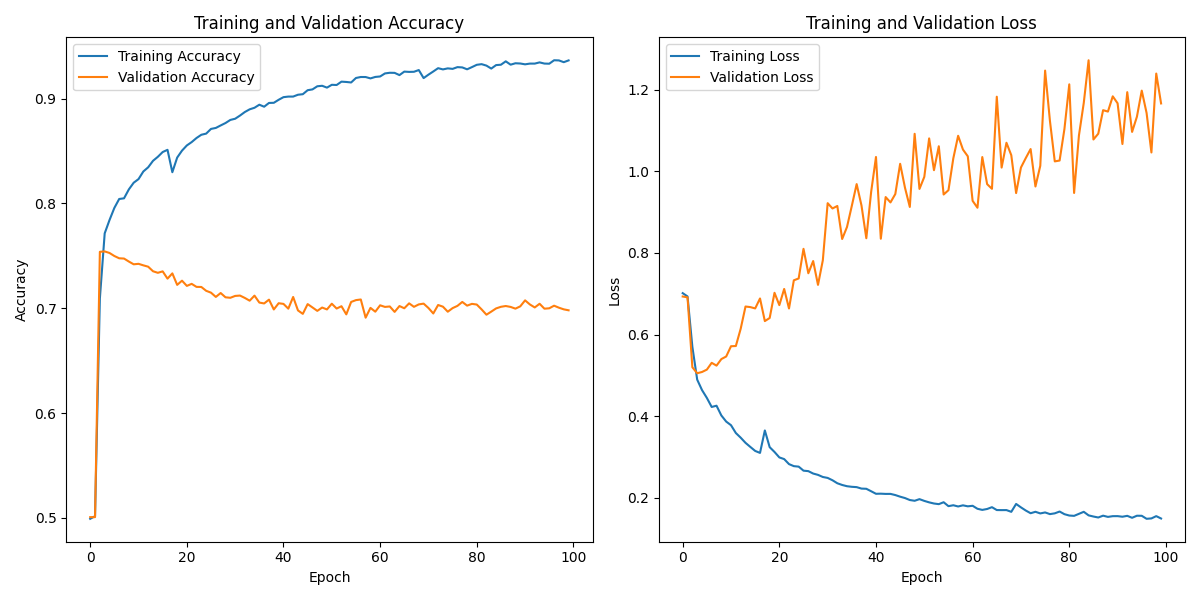
\includegraphics[width=1\linewidth]{Results/RNN/rnn1.png}
	\caption{ 1ο μοντέλο RNN }
	\label{f:g1}	
\end{figure}


\begin{figure}[ht]
	\centering
	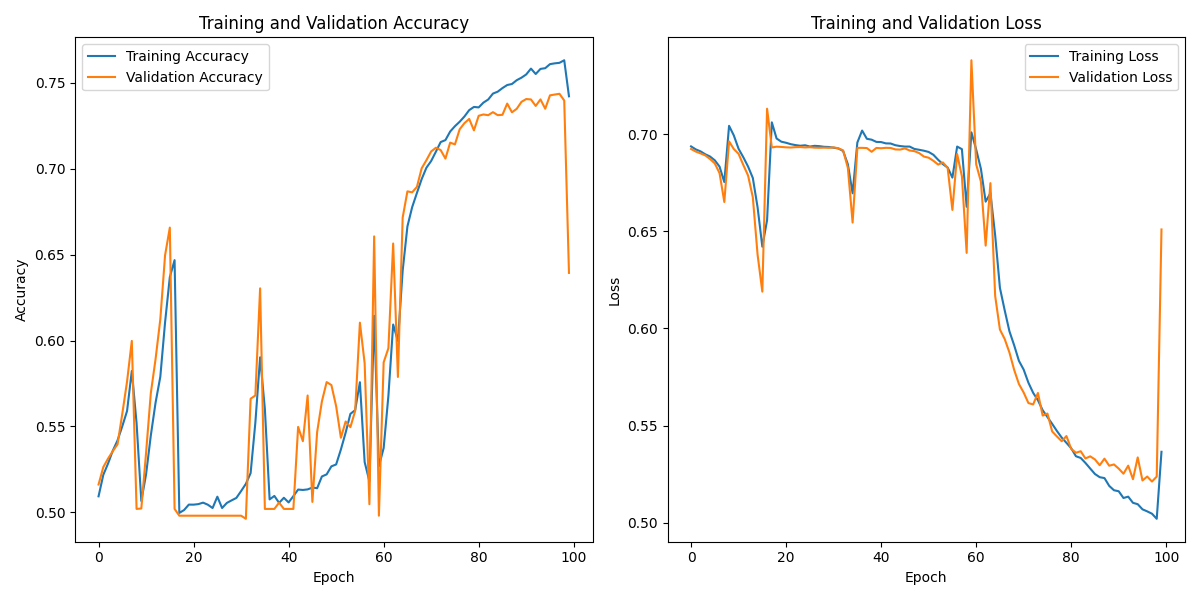
\includegraphics[width=1\linewidth]{Results/RNN/rnn2.png}
	\caption{ 2ο μοντέλο RNN }
	\label{f:g2}	
\end{figure}

\begin{figure}[ht]
	\centering
	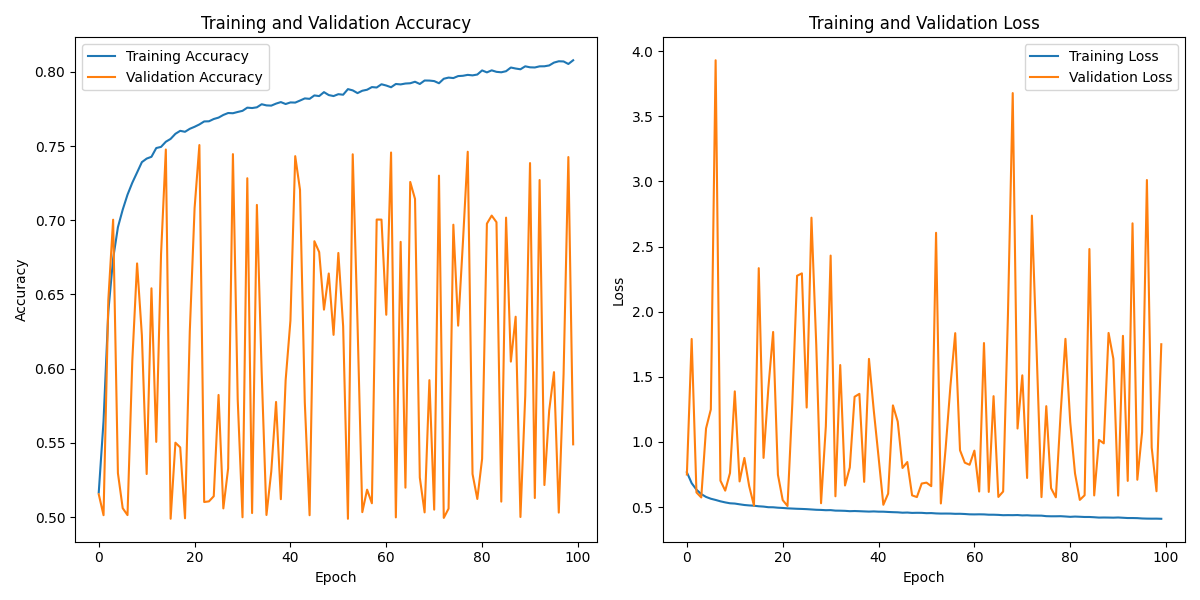
\includegraphics[width=1\linewidth]{Results/RNN/rnn3.png}
	\caption{ 3ο μοντέλο RNN}
	\label{f:g3}	
\end{figure}

\begin{figure}[ht]
	\centering
	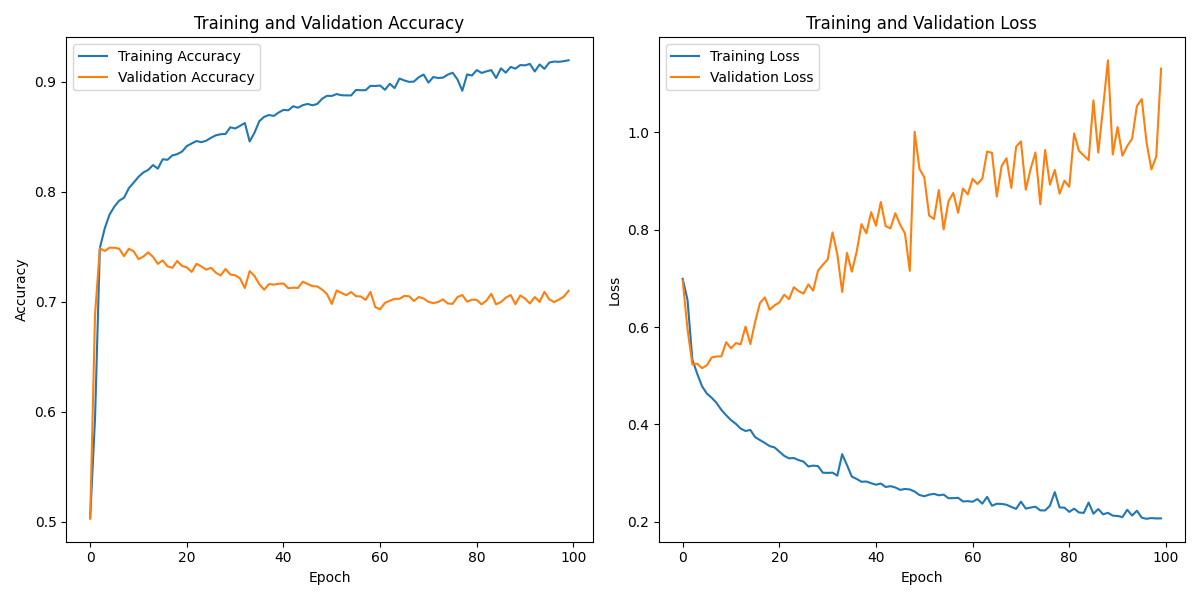
\includegraphics[width=1\linewidth]{Results/RNN/rnn4.png}
	\caption{ 4ο μοντέλο RNN }
	\label{f:g4}	
\end{figure}

\clearpage

\section{Συγκριση LSTM μοντέλων}

Στην συνένεχεια παρατηρήθηκαν παρόμοια αποτελέσματα στις εκπαιδεύσεις με των RNN, ειδικά στην 1η , 3η , 5η και 6η περίπτωση. Τα αντίστοιχα διαγράμματα τους έχουν σχεδόν την ίδια συμπεριφορά, με αυτήν των RNN. Από την άλλη στην 2η περίπτωση το μοντέλο έχει εκπαιδευτεί αρκετά καλα, παρόλο που το accuracy του ανεβαίνει μέχρι το 75$\%$, όπως φαίνεται και στο διάγραμμα \ref{f:g6}. Για αυτό τον λόγο έγινε μία προσπάθεια στην 4η περίπτωση με την εισαγωγή του Batch Normalization να αυξηθεί το accuracy αλλά παρατηρληθηκε και εδώ \ref{f:g8} ασταθής συμπεριφορά στο test accuracy/loss. Στο 5ο και στο 6ο με την άυξηση του learning rate και την μείωση του test dataset κατέληξε το μοντέλο σε overfitting \ref{f:g9}. Τέλος με την εισαγωγή του data augmentation το μοντέλο δεν μπορέσε να εκπαιδευτει και παρέμενιε στο 50$\%$ και το loss δεν έπεσε ποτέ \ref{f:g11}
,
\begin{figure}[ht]
	\centering
	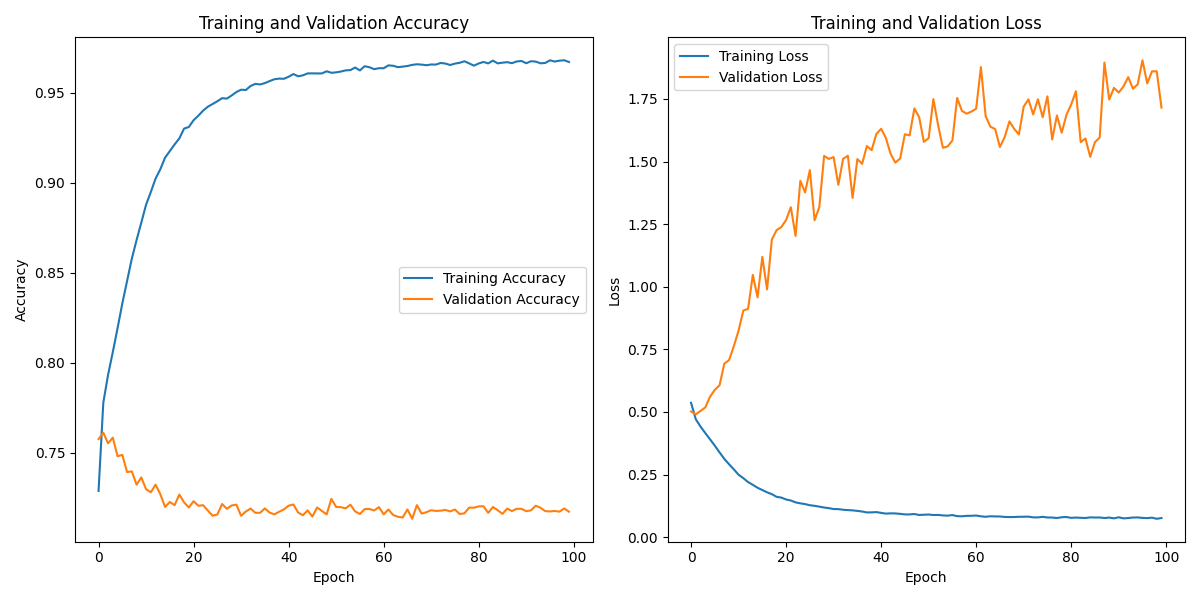
\includegraphics[width=1\linewidth]{Results/LSTM/lstm1.png}
	\caption{ 1ο μοντέλο LSTM}
	\label{f:g5}	
\end{figure}

\begin{figure}[ht]
	\centering
	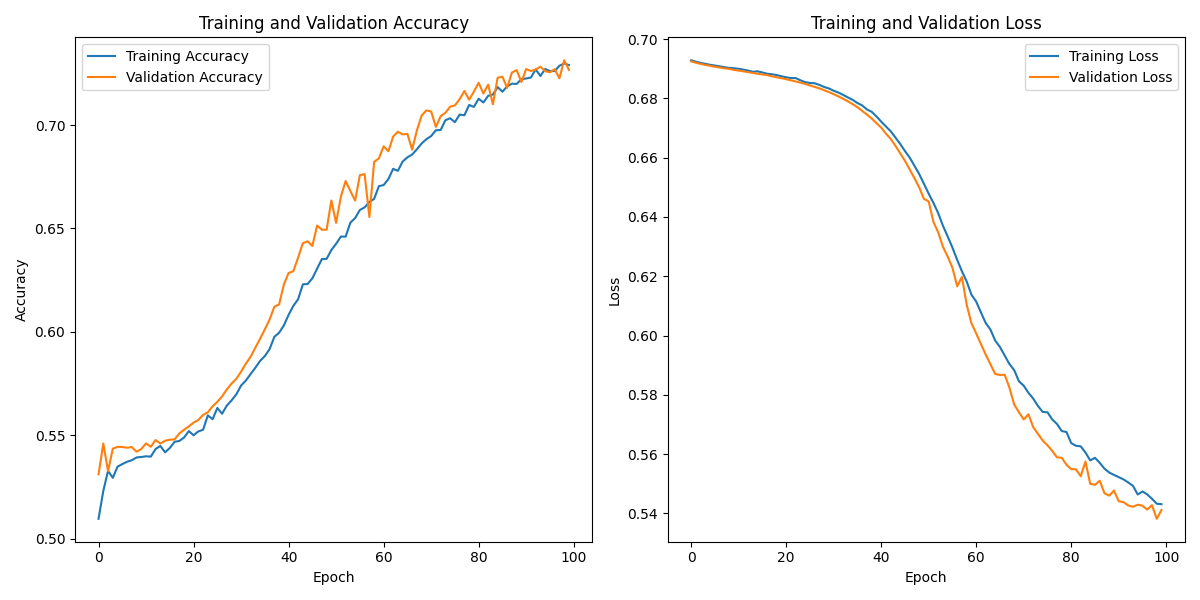
\includegraphics[width=1\linewidth]{Results/LSTM/lstm2.png}
	\caption{ 2ο μοντέλο LSTM}
	\label{f:g6}	
\end{figure}

\begin{figure}[ht]
	\centering
	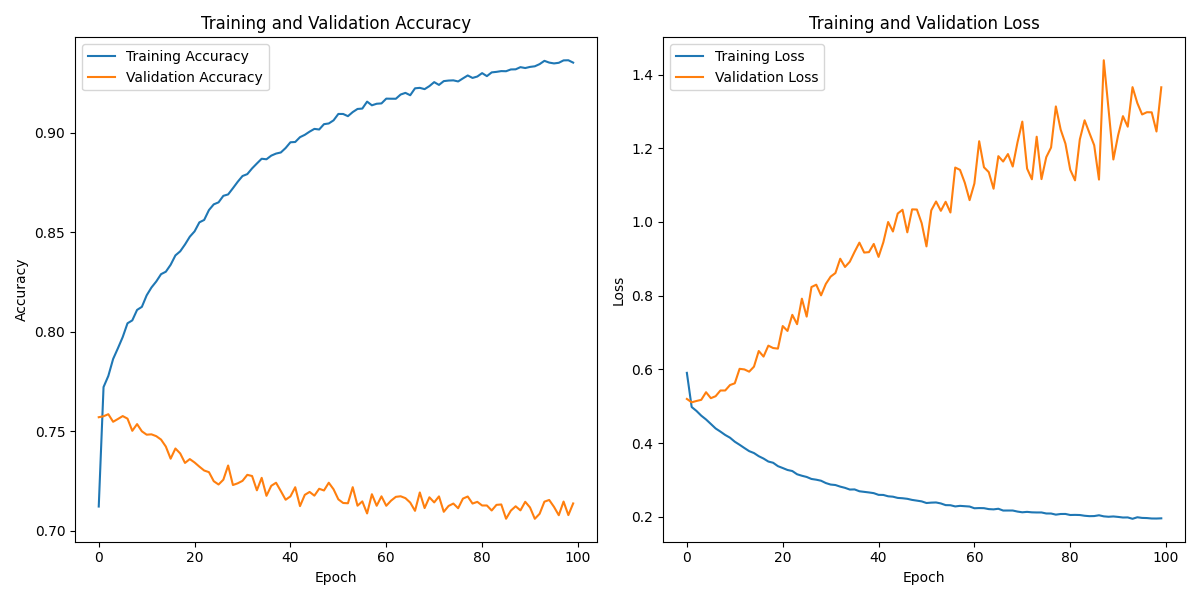
\includegraphics[width=1\linewidth]{Results/LSTM/lstm3.png}
	\caption{ 3ο μοντέλο LSTM}
	\label{f:g7}	
\end{figure}

\begin{figure}[ht]
	\centering
	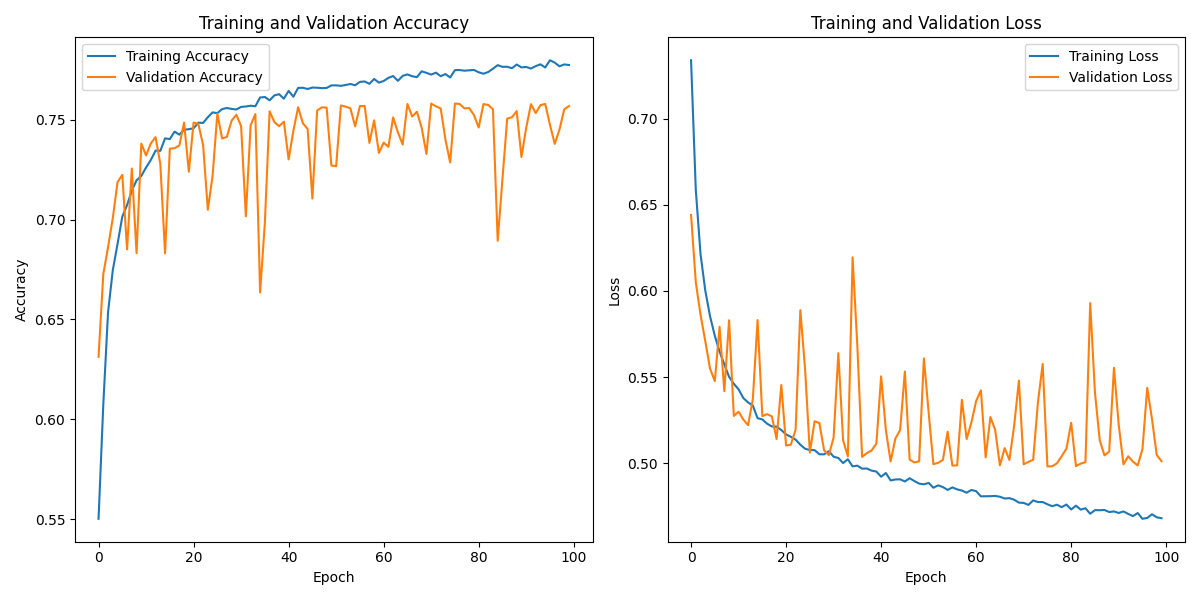
\includegraphics[width=1\linewidth]{Results/LSTM/lstm4.png}
	\caption{ 4ο μοντέλο LSTM}
	\label{f:g8}	
\end{figure}

\begin{figure}[ht]
	\centering
	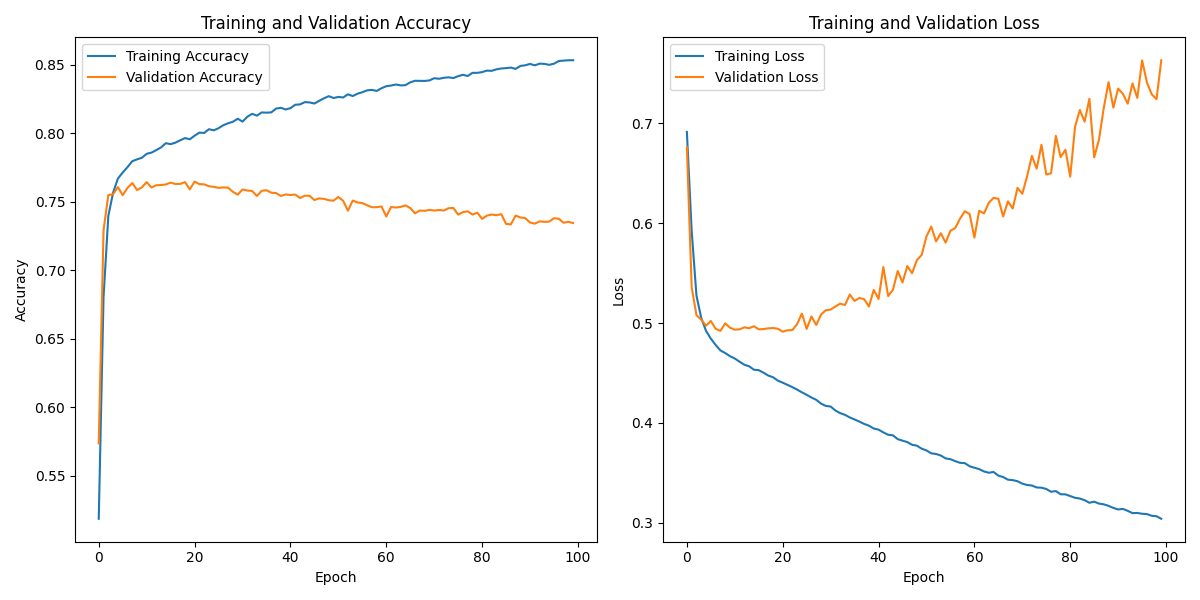
\includegraphics[width=1\linewidth]{Results/LSTM/lstm5.png}
	\caption{ 5ο μοντέλο LSTM}
	\label{f:g9}	
\end{figure}

\begin{figure}[ht]
	\centering
	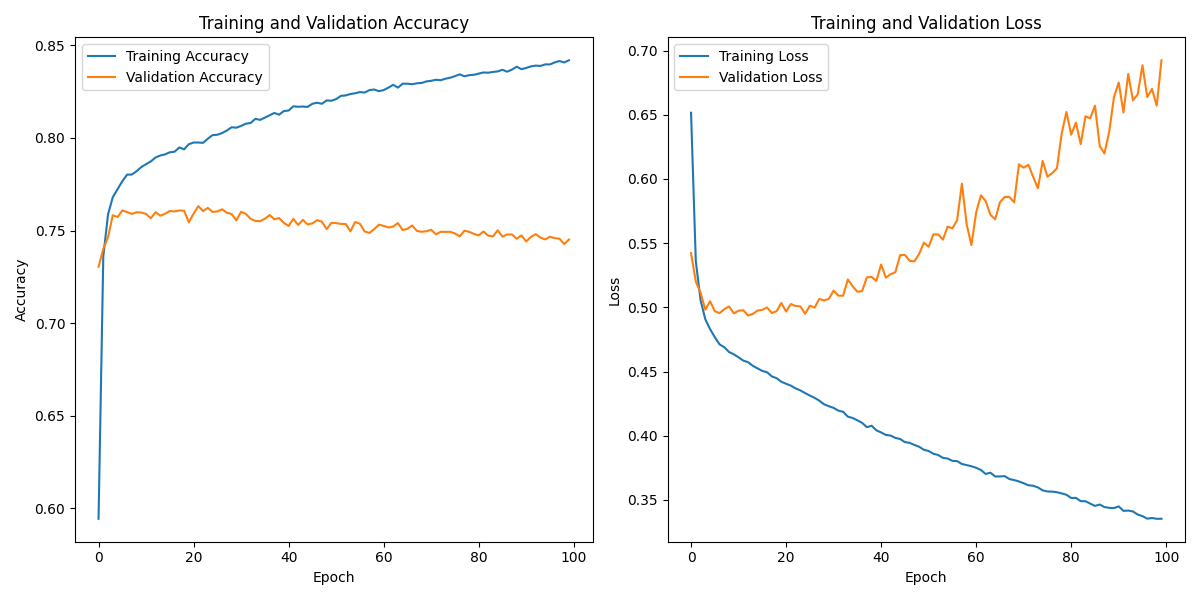
\includegraphics[width=1\linewidth]{Results/LSTM/lstm6.png}
	\caption{ 6ο μοντέλο LSTM}
	\label{f:g10}	
\end{figure}

\begin{figure}[ht]
	\centering
	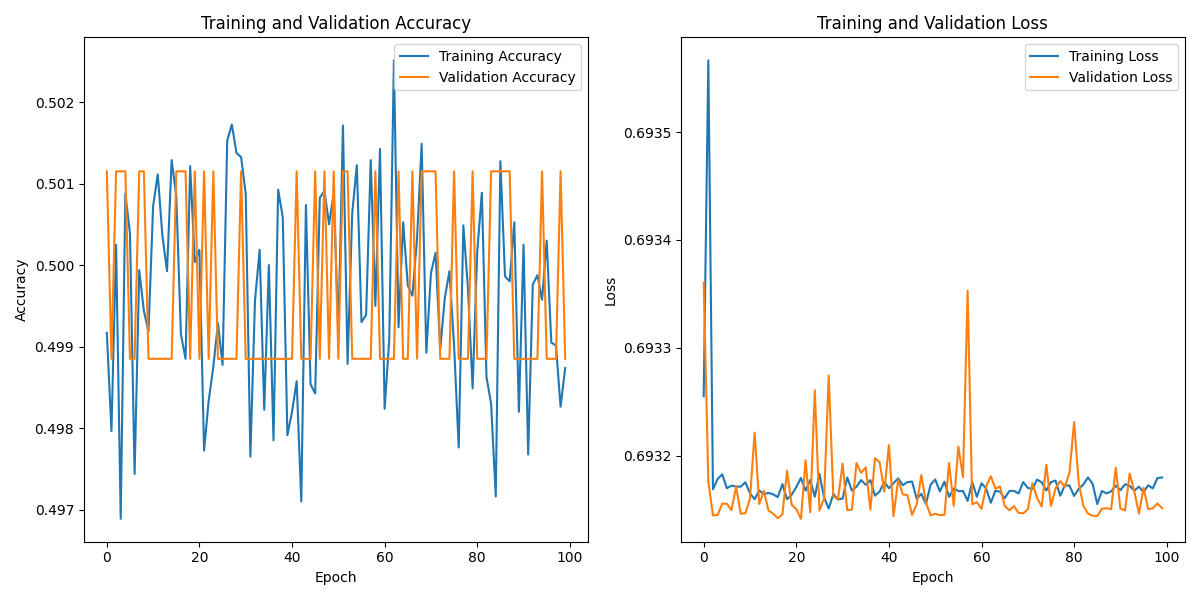
\includegraphics[width=1\linewidth]{Results/LSTM/lstm7.png}
	\caption{ 6ο μοντέλο LSTM}
	\label{f:g11}	
\end{figure}

\clearpage

\section{LSTM vs RNN}

Παρόλο που τα περισσότερα μοντέλα και στις 2 περιπτώσεις ήταν ασταθή τα LSTM είχαν καλύτερα αποτελέσματα κατι που περιμέναμε λόγω της αρχιτεκτονικής των LSTM. Tέλος τα spikes που παρατηρούνται στα περισσότερα μοντέλα υποδηλώνουν exploding gradients το οποίο μπορεί να οδηγήσει σε αριθμητική αστάθεια και να εμποδίσει την ικανότητα του μοντέλου να μάθει αποτελεσματικά, ακόμα και άν αυτό είναι πιο σταθερό αρχιτεκτονικά (LSTM).